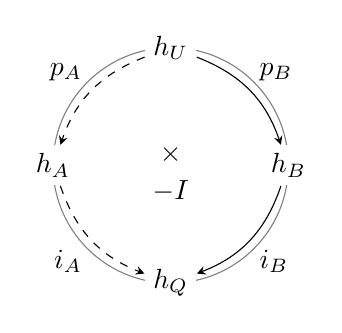
\begin{tikzpicture}[scale=1.15,>=stealth]
  \draw[gray] (0,0) circle (1.3);
  \node[fill=white,inner sep=3pt] (u) at (0,1.3) {$h_U$};
  \node[fill=white,inner sep=3pt] (b) at (1.3,0) {$h_B$};
  \node[fill=white,inner sep=3pt] (q) at (0,-1.3) {$h_Q$};
  \node[fill=white,inner sep=3pt] (a) at (-1.3,0) {$h_A$};
  \draw[->] (u) to[bend left=25] node[above right] {$p_B$} (b);
  \draw[->] (b) to[bend left=25] node[below right] {$i_B$} (q);
  \draw[->,dashed] (u) to[bend right=25] node[above left] {$p_A$} (a);
  \draw[->,dashed] (a) to[bend right=25] node[below left] {$i_A$} (q);
  \node at (0,0.12) {$\times$};
  \node at (0,-0.28) {$-I$};
\end{tikzpicture}
